\documentclass{article}
\usepackage[UTF8]{ctex}
% Replace `letterpaper' with`a4paper' for UK/EU standard size
\usepackage[a4paper,top=2cm,bottom=2cm,left=3cm,right=3cm,marginparwidth=1.75cm]{geometry}

% Useful packages
\usepackage{amsmath}
\usepackage{graphicx}
\usepackage[colorlinks=true, allcolors=blue]{hyperref}
\usepackage{graphicx} %插入图片的宏包
\usepackage{float} %设置图片浮动位置的宏包
\usepackage{subfigure} %插入多图时用子图显示的宏包
\usepackage{parskip}
\usepackage{indentfirst} 
\setlength{\parindent}{2em}
\usepackage{hyperref}  
\usepackage{tikz}
\allowdisplaybreaks
\usepackage{multirow}
\usepackage{amsmath}
\usepackage{amsfonts,amssymb} 
\usepackage{xcolor} % 用于显示颜色
\usepackage{listings} % 用于插入代码
\lstset{
	basicstyle          =   \sffamily,          % 基本代码风格
	keywordstyle        =   \bfseries,          % 关键字风格
	commentstyle        =   \rmfamily\itshape,  % 注释的风格,斜体
	stringstyle         =   \ttfamily,  % 字符串风格
	flexiblecolumns,                % 别问为什么,加上这个
	numbers             =   left,   % 行号的位置在左边
	showspaces          =   false,  % 是否显示空格,显示了有点乱,所以不现实了
	numberstyle         =   \zihao{-5}\ttfamily,    % 行号的样式,小五号,tt等宽字体
	showstringspaces    =   false,
	captionpos          =   t,      % 这段代码的名字所呈现的位置,t指的是top上面
	frame               =   lrtb,   % 显示边框
}

\lstdefinestyle{Python}{
	language        =   Python, % 语言选Python
	basicstyle      =   \zihao{-5}\ttfamily,
	numberstyle     =   \zihao{-5}\ttfamily,
	keywordstyle    =   \color{blue},
	keywordstyle    =   [2] \color{teal},
	stringstyle     =   \color{magenta},
	commentstyle    =   \color{red}\ttfamily,
	breaklines      =   true,   % 自动换行,建议不要写太长的行
	columns         =   fixed,  % 如果不加这一句,字间距就不固定,很丑,必须加
	basewidth       =   0.5em,
}

\title{Project-1 Pacman实验报告}
\author{陈笑宇 21340246003$\quad$林子开 21307110161}
\date{}
\begin{document}
	\maketitle
%	\tableofcontents

\section{使用深度优先搜索找到固定的食物点}
在本题中,使用深度优先搜索(DFS),并且使用util文件中的Stack作为维护“后进先出”的数据结构,
将从起点到该点的路径加上到达下一个点的action作为path,
与下一个点一起压入Stack中。此外,我们使用explored列表,来保证
不再访问那些已经访问过的节点。

请注意!\textbf{在我们以下的所有的算法中,我们都规定在某个节点弹出frontier的时候,
才对其判断是否为目标节点。
因此,我们的算法可能比其他先判断是否为goal,然后再入frontier的算法多扩展一些节点。}

我们的实验结果如下:

\begin{table}[H]
	\centering
	\caption{DFS实验结果}
	\begin{tabular}{lll}
	\hline
	迷宫类型       & 扩展的节点 & 代价  \\
	\hline
	TinyMaze   & 15    & 10  \\
	MediumMaze & 146   & 130 \\
	BigMaze    & 390   & 210\\
	\hline
	\end{tabular}
	\end{table}

\section{广度优先搜索}
在本题中,使用广度优先搜索(BFS),并且使用util文件中的Queue作为维护“先进先出”的数据结构,
同样将到达下一个点的path和下一个点一起推入Queue中。类似的,我们也使用explored列表
来防止重复访问。我们的实验结果如下:
\begin{table}[H]
	\centering
	\caption{BFS实验结果}
	\begin{tabular}{lll}
		\hline
	迷宫类型       & 扩展的节点 & 代价  \\ \hline
	TinyMaze   & 15    & 8   \\
	MediumMaze & 269   & 68  \\
	BigMaze    & 620   & 210 \\ \hline
	\end{tabular}
	\end{table}


\section{一致代价搜索}
在本题中,我们使用util中的优先队列PriorityQueue来保证最低代价节点先被访问。
我们将下一个节点、到达下一个节点的path,以及这条path的cost作为一个三元组
推入优先队列中。

其中,path的cost通过getCostOfActions函数计算得到。
我们的实验结果如下:

\begin{table}[H]
	\centering
	\caption{UCS实验结果}
	\begin{tabular}{lll}
		\hline
	迷宫类型             & 扩展的节点 & 代价          \\
	\hline
	MediumMaze       & 270   & 68          \\
	MediumDottedMaze & 187   & 1           \\
	MeidumScaryMaze  & 108   &  68719479864 \\
	\hline
	\end{tabular}
	\end{table}


\section{A*搜索}
在本题中,我们在构建A*搜索时,我们将从起点到下一个点的cost与启发式函数的估计值相加,
将其作为权重,推入优先队列PriorityQueue中。在本题中,我们统一使用曼哈顿距离启发式进行测试。
我们在bigMaze上测试了DFS,BFS,UCS和A*,实验结果如下:

\begin{table}[H]
	\centering
	\caption{在bigMaze上测试DFS,BFS,UCS和A*的实验结果}
	\begin{tabular}{lll}
		\hline
	迷宫类型                           & 扩展的节点 & 代价  \\
	\hline
	dfs                            & 390   & 210 \\
	bfs                            & 620   & 210 \\
	ucs                            & 621   & 210 \\
	astar(with manhattanHeuristic) & 549   & 210\\ \hline
	\end{tabular}
	\end{table}

	可以看出,A*比UCS扩展的节点略少一点。现在,我们继续在openMaze测试上述四种搜索策略:

	\begin{table}[H]
		\centering
		\caption{在openMaze上测试DFS,BFS,UCS和A*的实验结果}
		\begin{tabular}{lll}
			\hline
		迷宫类型                           & 扩展的节点 & 代价  \\ \hline
		dfs                            & 576   & 298 \\
		bfs                            & 682   & 54  \\
		ucs                            & 683   & 54  \\
		astar(with manhattanHeuristic) & 535   & 54 \\ \hline
		\end{tabular}
		\end{table}

可以发现,DFS在openmaze上并没有找到最优解。BFS,UCS,A*都找到了最优解,但是A*算法
扩展的节点仍然比BFS和UCS更少。

\section{找到所有角落}
在本题中,我们将当前的坐标以及已经访问过的角落作为state。
其中,我们\textbf{用一个列表来存储已经访问过的角落}。
在判断是否为目标状态的isGoalState函数中,以及得到下一个状态的getSuccessors函数中,
我们用相同的方法来判断和更新已访问角落的信息。

我们首先判断当前点的坐标是否为角落;如果该坐标是角落,再判断是否为一个不曾访问过的角落;
如果确实是一个不曾访问过的角落,则将信息更新,也即向记录已访问角落的列表中加入该坐标。
\textbf{当该列表的长度到达4,也即所有的角落都访问过时,我们认为已经达到目标状态}。

现在,使用BFS策略,我们已经能够解决找到所有角落问题。实验结果如下:
\begin{table}[H]
	\centering
	\caption{使用BFS找到所有角落的实验结果}
	\begin{tabular}{lll}
		\hline
	迷宫类型          & 扩展的节点 & 代价  \\ \hline
	tinyCorners   & 435   & 28  \\
	mediumCorners & 2448  & 106\\ \hline
	\end{tabular}
	\end{table}

\section{使用带启发式的A*策略找到所有角落}
我们使用的启发式\textbf{基于问题松弛}。也即,假设没有围墙,到达距离吃豆人最近角落
的曼哈顿距离。示意图如下:
\begin{figure}[H]
	\centering
	{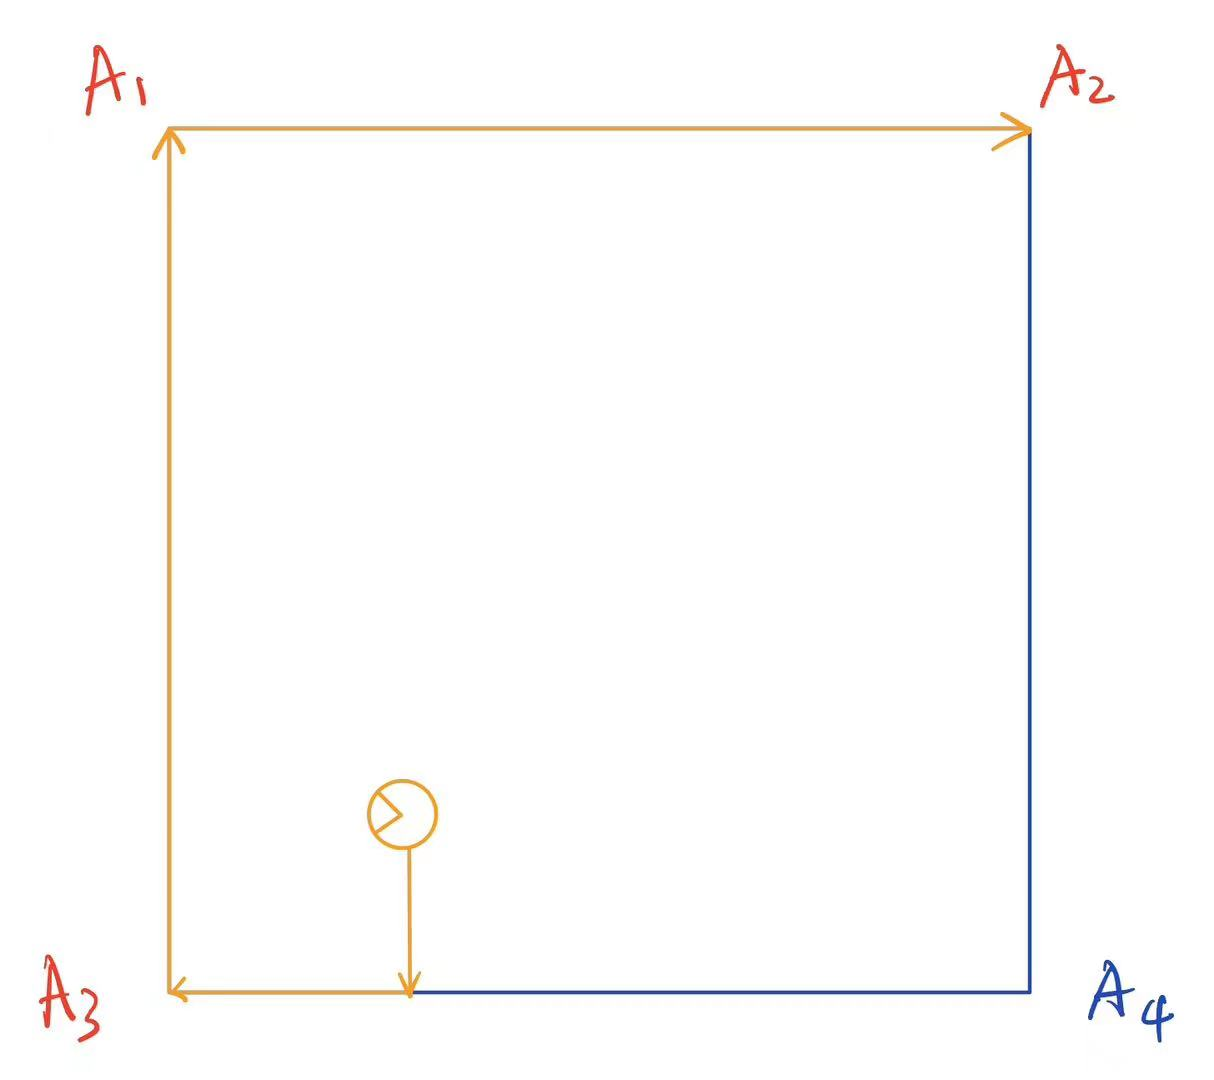
\includegraphics[width=0.3\textwidth]{image//启发式示意图.jpg}} 
	\caption{所采用的启发式的示意图}\label{Hfunc}
\end{figure}

在示意图中\ref{Hfunc}中,我们假设没有围墙,且已经访问过A4角落,未访问过A1,A2和A3角落,
那么,启发式即等于吃豆人前往角落A3的曼哈顿距离。

这个启发式显然是\textbf{可采纳的},因为无论如何,吃豆人最后都会到达这个目前距离自己最近的角落,
且在任何有围墙的情况下的路程cost,必定会大于或等于松弛问题下直接前往最近角落的cost。

此外,我们的启发式也是\textbf{一致的},
我们仍然以图\ref{Hfunc}为例进行说明。假设当前位置到A1,A2,A3角落的曼哈顿距离分别为
$S_1,S_2,S_3$,那么,并且有$S_3 \le S_1 \le S_2$,在进行曼哈顿距离为$c$的移动之后,
到达三个角落的距离分别为$X_1,X_2,X_3$,并且应该会满足$X_i \ge S_i-c\, ,\, i=1,2,3$。
若仍然距离A3最近,则显然启发值最多能降低c,因为$c \ge S_3-X_3$。
若距离其他角落更近,我们不妨设距离A1更近,那么$S_3-X_1 \le S_3-S_1+c \le c$,
也即启发值最多降低c。
至此,我们证明了该启发式是一致的。


我们的实验结果如下:

\begin{table}[H]
	\centering
	\caption{使用UCS和A*找到所有角落的实验结果}
	\begin{tabular}{llll}
		\hline
	迷宫类型          & 搜索策略                              & 扩展的节点 & 代价  \\ \hline
	mediumCorners &  A*(with our own cornersHeuristic)    & 1745  & 106 \\
	mediumCorners & UCS & 2449  & 106 \\ \hline
	\end{tabular}
	\end{table}


注意到,使用A*所得到的路径长度与使用UCS所得到的路径长度相同,都是106,
这也进一步验证了我们给出的启发式是可采纳的且一致的。

\section{吃掉所有的点}
我们使用的启发式为:
以当前位置作为起点,再分别以所有剩余食物作为终点,利用PositionSearchProblem定义
一个新的搜索问题,用BFS寻找到最短路径。然后我们将到达各个食物的最短路径中的最大值
(也即到最远食物的距离)作为启发值。

这个启发式是\textbf{一致的},证明如下:
假设当前吃豆人所在位置是X,距离最远(在最短路径意义下)的食物的位置是Y,那么,X位置的
启发值即为从X到Y的路径长度$S_{XY}$。当吃豆人移动了$c$的路径程度到达了新的位置Z,此时Z到
食物Y的距离满足$S_{ZY} \ge S_{XY} - c$。如果此时距离位置Z最远的食物仍然是Y处的食物,
那么Z处的启发值显然满足$  S_{XY} - S_{ZY} \le c$。
若此时距离位置Z最远的不是Y,而是W处的食物,那么应该满足$S_{ZY} < S_{ZW}$,显然也有
$  S_{XY} - S_{ZW} \le c$。综上,不论吃豆人在移动后距离最远食物是Y还是W,启发值最多都
只可能下降$c$。至此,我们证明了我们给出的启发式是一致的。


我们的实验结果如下:
\begin{table}[H]
	\centering
	\caption{带启发式的A*搜索在trickySearch上的实验结果}
	\begin{tabular}{llll}
		\hline
	迷宫类型         & 扩展的节点 & 代价 & 探索时间 \\ \hline
	trickySearch & 4110  & 60 & 21.5 \\ \hline
	\end{tabular}
	\end{table}

\section{次优搜索}
在本题中,我们总是使用BFS找到距离吃豆人最近的食物。
我们对bigSearch进行搜索,迅速得到了一条cost为350的路径。
但是,在这条路径中,吃豆人忽略了右侧的一个食物,最后还要回到迷宫右侧,
这严重导致了该路径的次优性,如下图所示:

\begin{figure}[H]
	\centering
	{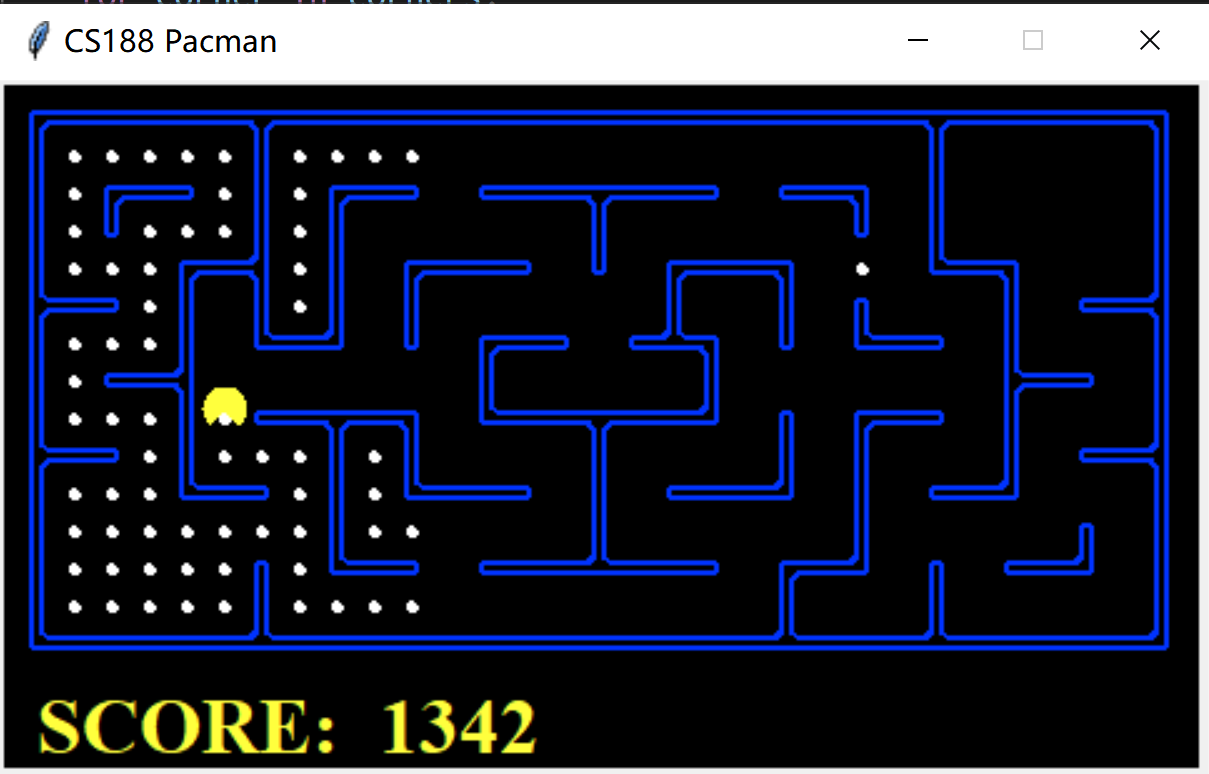
\includegraphics[width=0.35\textwidth]{image//ignorance.png}} 
	\caption{次优路径忽略了右侧的一个点}
\end{figure}

下面,我们给出一个简单的一维空间上例子,说明重复前往最近的点,
并不会找到吃掉所有点的最短路径,如下所示:
\begin{figure}[H]
	\centering
	{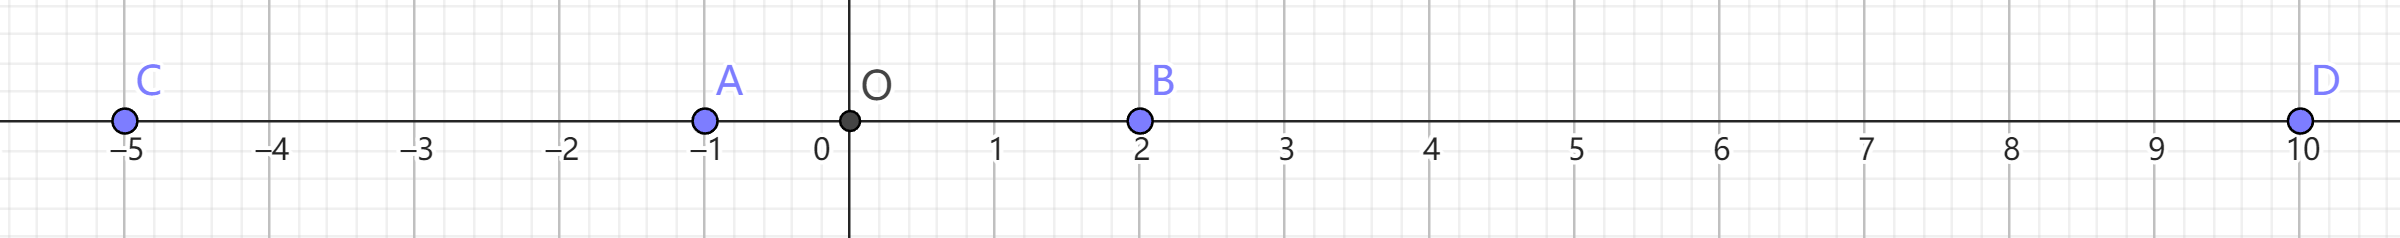
\includegraphics[width=0.7\textwidth]{image//example.png}} 
	\caption{一个说明贪婪策略无法找到全局最优解的一维例子}
\end{figure}
在这个例子中,如果使用贪心算法,不断前往最近的点,则吃豆人的路径应该为$O\to A \to B \to C \to D$,
这条路径的长度为$1+3+7+15=26$。
但实际上,这条路径缺乏对全局信息的掌握,反复在中间部分来回行走,导致其不是最优。
如果使用BFS或UCS或A*等算法,可以发现最优路径应该是$O \to A \to C \to B \to D$,
相应的总路径长度是$1+4+7+8 =20$。


\end{document}